% Created by tikzDevice version 0.12.6 on 2024-06-15 18:35:23
% !TEX encoding = UTF-8 Unicode
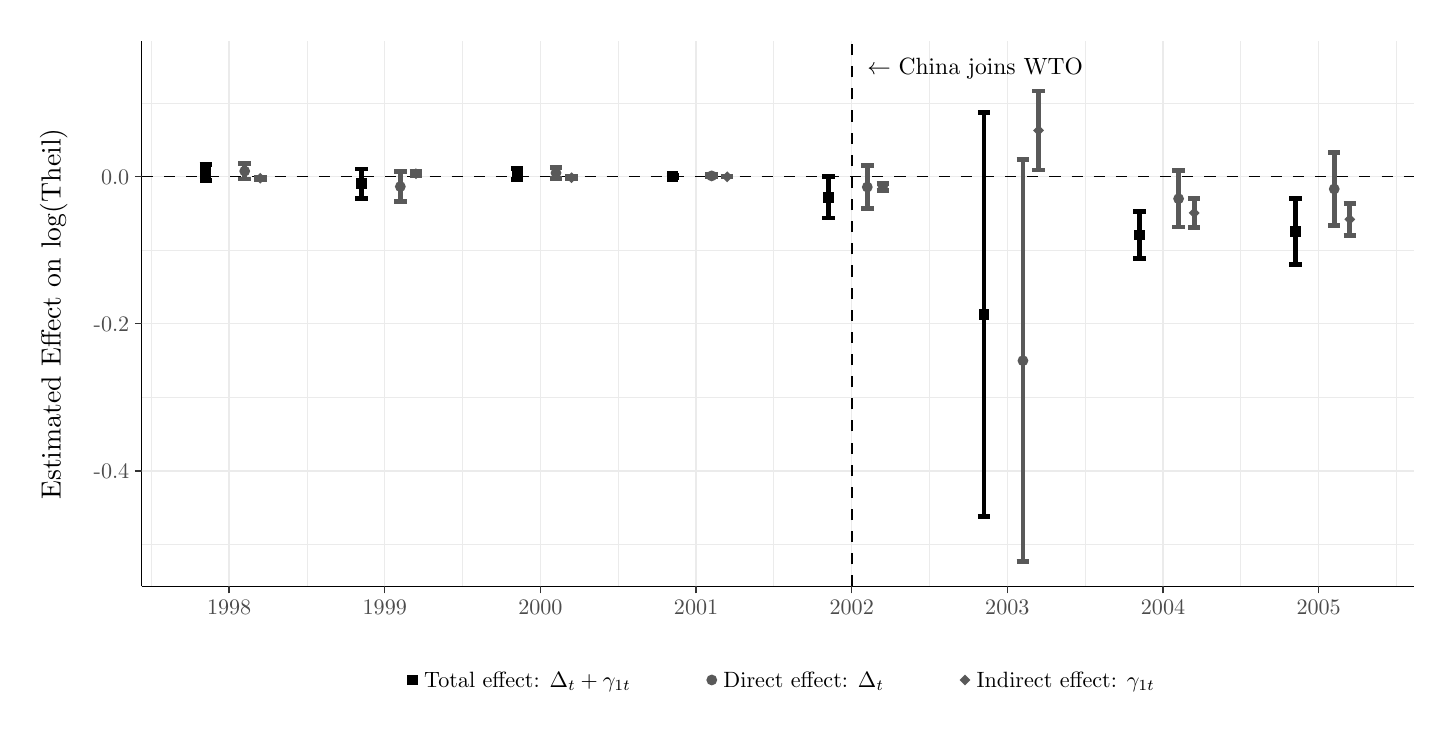
\begin{tikzpicture}[x=1pt,y=1pt]
\definecolor{fillColor}{RGB}{255,255,255}
\path[use as bounding box,fill=fillColor] (0,0) rectangle (505.89,252.94);
\begin{scope}
\path[clip] (  0.00,  0.00) rectangle (505.89,252.94);
\definecolor{drawColor}{RGB}{255,255,255}

\path[draw=drawColor,line width= 0.5pt,line join=round,line cap=round,fill=fillColor] (  0.00, -0.00) rectangle (505.89,252.94);
\end{scope}
\begin{scope}
\path[clip] ( 41.22, 51.02) rectangle (500.89,247.95);
\definecolor{fillColor}{RGB}{255,255,255}

\path[fill=fillColor] ( 41.22, 51.02) rectangle (500.89,247.95);
\definecolor{drawColor}{gray}{0.92}

\path[draw=drawColor,line width= 0.3pt,line join=round] ( 41.22, 66.18) --
	(500.89, 66.18);

\path[draw=drawColor,line width= 0.3pt,line join=round] ( 41.22,119.35) --
	(500.89,119.35);

\path[draw=drawColor,line width= 0.3pt,line join=round] ( 41.22,172.53) --
	(500.89,172.53);

\path[draw=drawColor,line width= 0.3pt,line join=round] ( 41.22,225.70) --
	(500.89,225.70);

\path[draw=drawColor,line width= 0.3pt,line join=round] ( 44.68, 51.02) --
	( 44.68,247.95);

\path[draw=drawColor,line width= 0.3pt,line join=round] (100.92, 51.02) --
	(100.92,247.95);

\path[draw=drawColor,line width= 0.3pt,line join=round] (157.16, 51.02) --
	(157.16,247.95);

\path[draw=drawColor,line width= 0.3pt,line join=round] (213.40, 51.02) --
	(213.40,247.95);

\path[draw=drawColor,line width= 0.3pt,line join=round] (269.65, 51.02) --
	(269.65,247.95);

\path[draw=drawColor,line width= 0.3pt,line join=round] (325.89, 51.02) --
	(325.89,247.95);

\path[draw=drawColor,line width= 0.3pt,line join=round] (382.13, 51.02) --
	(382.13,247.95);

\path[draw=drawColor,line width= 0.3pt,line join=round] (438.38, 51.02) --
	(438.38,247.95);

\path[draw=drawColor,line width= 0.3pt,line join=round] (494.62, 51.02) --
	(494.62,247.95);

\path[draw=drawColor,line width= 0.5pt,line join=round] ( 41.22, 92.76) --
	(500.89, 92.76);

\path[draw=drawColor,line width= 0.5pt,line join=round] ( 41.22,145.94) --
	(500.89,145.94);

\path[draw=drawColor,line width= 0.5pt,line join=round] ( 41.22,199.11) --
	(500.89,199.11);

\path[draw=drawColor,line width= 0.5pt,line join=round] ( 72.80, 51.02) --
	( 72.80,247.95);

\path[draw=drawColor,line width= 0.5pt,line join=round] (129.04, 51.02) --
	(129.04,247.95);

\path[draw=drawColor,line width= 0.5pt,line join=round] (185.28, 51.02) --
	(185.28,247.95);

\path[draw=drawColor,line width= 0.5pt,line join=round] (241.53, 51.02) --
	(241.53,247.95);

\path[draw=drawColor,line width= 0.5pt,line join=round] (297.77, 51.02) --
	(297.77,247.95);

\path[draw=drawColor,line width= 0.5pt,line join=round] (354.01, 51.02) --
	(354.01,247.95);

\path[draw=drawColor,line width= 0.5pt,line join=round] (410.25, 51.02) --
	(410.25,247.95);

\path[draw=drawColor,line width= 0.5pt,line join=round] (466.50, 51.02) --
	(466.50,247.95);
\definecolor{drawColor}{RGB}{0,0,0}

\path[draw=drawColor,line width= 0.6pt,dash pattern=on 4pt off 4pt ,line join=round] ( 41.22,199.11) -- (500.89,199.11);

\path[draw=drawColor,line width= 0.6pt,dash pattern=on 4pt off 4pt ,line join=round] (297.77, 51.02) -- (297.77,247.95);

\node[text=drawColor,anchor=base west,inner sep=0pt, outer sep=0pt, scale=  0.85] at (303.39,236.05) {$\leftarrow$ China joins WTO};

\path[draw=drawColor,line width= 1.7pt,line join=round] ( 62.11,203.43) --
	( 66.61,203.43);

\path[draw=drawColor,line width= 1.7pt,line join=round] ( 64.36,203.43) --
	( 64.36,197.61);

\path[draw=drawColor,line width= 1.7pt,line join=round] ( 62.11,197.61) --
	( 66.61,197.61);

\path[draw=drawColor,line width= 1.7pt,line join=round] (118.35,201.87) --
	(122.85,201.87);

\path[draw=drawColor,line width= 1.7pt,line join=round] (120.60,201.87) --
	(120.60,191.27);

\path[draw=drawColor,line width= 1.7pt,line join=round] (118.35,191.27) --
	(122.85,191.27);

\path[draw=drawColor,line width= 1.7pt,line join=round] (174.60,202.05) --
	(179.10,202.05);

\path[draw=drawColor,line width= 1.7pt,line join=round] (176.85,202.05) --
	(176.85,198.06);

\path[draw=drawColor,line width= 1.7pt,line join=round] (174.60,198.06) --
	(179.10,198.06);

\path[draw=drawColor,line width= 1.7pt,line join=round] (230.84,199.69) --
	(235.34,199.69);

\path[draw=drawColor,line width= 1.7pt,line join=round] (233.09,199.69) --
	(233.09,198.92);

\path[draw=drawColor,line width= 1.7pt,line join=round] (230.84,198.92) --
	(235.34,198.92);

\path[draw=drawColor,line width= 1.7pt,line join=round] (287.08,199.12) --
	(291.58,199.12);

\path[draw=drawColor,line width= 1.7pt,line join=round] (289.33,199.12) --
	(289.33,184.19);

\path[draw=drawColor,line width= 1.7pt,line join=round] (287.08,184.19) --
	(291.58,184.19);

\path[draw=drawColor,line width= 1.7pt,line join=round] (343.33,222.22) --
	(347.83,222.22);

\path[draw=drawColor,line width= 1.7pt,line join=round] (345.58,222.22) --
	(345.58, 76.39);

\path[draw=drawColor,line width= 1.7pt,line join=round] (343.33, 76.39) --
	(347.83, 76.39);

\path[draw=drawColor,line width= 1.7pt,line join=round] (399.57,186.51) --
	(404.07,186.51);

\path[draw=drawColor,line width= 1.7pt,line join=round] (401.82,186.51) --
	(401.82,169.51);

\path[draw=drawColor,line width= 1.7pt,line join=round] (399.57,169.51) --
	(404.07,169.51);

\path[draw=drawColor,line width= 1.7pt,line join=round] (455.81,191.09) --
	(460.31,191.09);

\path[draw=drawColor,line width= 1.7pt,line join=round] (458.06,191.09) --
	(458.06,167.33);

\path[draw=drawColor,line width= 1.7pt,line join=round] (455.81,167.33) --
	(460.31,167.33);
\definecolor{drawColor}{gray}{0.35}

\path[draw=drawColor,line width= 1.7pt,line join=round] ( 76.17,203.94) --
	( 80.67,203.94);

\path[draw=drawColor,line width= 1.7pt,line join=round] ( 78.42,203.94) --
	( 78.42,198.26);

\path[draw=drawColor,line width= 1.7pt,line join=round] ( 76.17,198.26) --
	( 80.67,198.26);

\path[draw=drawColor,line width= 1.7pt,line join=round] (132.41,200.98) --
	(136.91,200.98);

\path[draw=drawColor,line width= 1.7pt,line join=round] (134.66,200.98) --
	(134.66,190.06);

\path[draw=drawColor,line width= 1.7pt,line join=round] (132.41,190.06) --
	(136.91,190.06);

\path[draw=drawColor,line width= 1.7pt,line join=round] (188.66,202.35) --
	(193.16,202.35);

\path[draw=drawColor,line width= 1.7pt,line join=round] (190.91,202.35) --
	(190.91,198.55);

\path[draw=drawColor,line width= 1.7pt,line join=round] (188.66,198.55) --
	(193.16,198.55);

\path[draw=drawColor,line width= 1.7pt,line join=round] (244.90,199.79) --
	(249.40,199.79);

\path[draw=drawColor,line width= 1.7pt,line join=round] (247.15,199.79) --
	(247.15,198.98);

\path[draw=drawColor,line width= 1.7pt,line join=round] (244.90,198.98) --
	(249.40,198.98);

\path[draw=drawColor,line width= 1.7pt,line join=round] (301.14,203.13) --
	(305.64,203.13);

\path[draw=drawColor,line width= 1.7pt,line join=round] (303.39,203.13) --
	(303.39,187.55);

\path[draw=drawColor,line width= 1.7pt,line join=round] (301.14,187.55) --
	(305.64,187.55);

\path[draw=drawColor,line width= 1.7pt,line join=round] (357.39,205.24) --
	(361.89,205.24);

\path[draw=drawColor,line width= 1.7pt,line join=round] (359.64,205.24) --
	(359.64, 59.97);

\path[draw=drawColor,line width= 1.7pt,line join=round] (357.39, 59.97) --
	(361.89, 59.97);

\path[draw=drawColor,line width= 1.7pt,line join=round] (413.63,201.40) --
	(418.13,201.40);

\path[draw=drawColor,line width= 1.7pt,line join=round] (415.88,201.40) --
	(415.88,180.86);

\path[draw=drawColor,line width= 1.7pt,line join=round] (413.63,180.86) --
	(418.13,180.86);

\path[draw=drawColor,line width= 1.7pt,line join=round] (469.87,207.88) --
	(474.37,207.88);

\path[draw=drawColor,line width= 1.7pt,line join=round] (472.12,207.88) --
	(472.12,181.41);

\path[draw=drawColor,line width= 1.7pt,line join=round] (469.87,181.41) --
	(474.37,181.41);

\path[draw=drawColor,line width= 1.7pt,line join=round] ( 81.80,199.02) --
	( 86.30,199.02);

\path[draw=drawColor,line width= 1.7pt,line join=round] ( 84.05,199.02) --
	( 84.05,198.05);

\path[draw=drawColor,line width= 1.7pt,line join=round] ( 81.80,198.05) --
	( 86.30,198.05);

\path[draw=drawColor,line width= 1.7pt,line join=round] (138.04,201.00) --
	(142.54,201.00);

\path[draw=drawColor,line width= 1.7pt,line join=round] (140.29,201.00) --
	(140.29,199.32);

\path[draw=drawColor,line width= 1.7pt,line join=round] (138.04,199.32) --
	(142.54,199.32);

\path[draw=drawColor,line width= 1.7pt,line join=round] (194.28,199.05) --
	(198.78,199.05);

\path[draw=drawColor,line width= 1.7pt,line join=round] (196.53,199.05) --
	(196.53,198.40);

\path[draw=drawColor,line width= 1.7pt,line join=round] (194.28,198.40) --
	(198.78,198.40);

\path[draw=drawColor,line width= 1.7pt,line join=round] (250.52,199.10) --
	(255.02,199.10);

\path[draw=drawColor,line width= 1.7pt,line join=round] (252.77,199.10) --
	(252.77,198.97);

\path[draw=drawColor,line width= 1.7pt,line join=round] (250.52,198.97) --
	(255.02,198.97);

\path[draw=drawColor,line width= 1.7pt,line join=round] (306.77,196.65) --
	(311.27,196.65);

\path[draw=drawColor,line width= 1.7pt,line join=round] (309.02,196.65) --
	(309.02,194.19);

\path[draw=drawColor,line width= 1.7pt,line join=round] (306.77,194.19) --
	(311.27,194.19);

\path[draw=drawColor,line width= 1.7pt,line join=round] (363.01,230.06) --
	(367.51,230.06);

\path[draw=drawColor,line width= 1.7pt,line join=round] (365.26,230.06) --
	(365.26,201.56);

\path[draw=drawColor,line width= 1.7pt,line join=round] (363.01,201.56) --
	(367.51,201.56);

\path[draw=drawColor,line width= 1.7pt,line join=round] (419.25,191.31) --
	(423.75,191.31);

\path[draw=drawColor,line width= 1.7pt,line join=round] (421.50,191.31) --
	(421.50,180.66);

\path[draw=drawColor,line width= 1.7pt,line join=round] (419.25,180.66) --
	(423.75,180.66);

\path[draw=drawColor,line width= 1.7pt,line join=round] (475.50,189.50) --
	(480.00,189.50);

\path[draw=drawColor,line width= 1.7pt,line join=round] (477.75,189.50) --
	(477.75,177.85);

\path[draw=drawColor,line width= 1.7pt,line join=round] (475.50,177.85) --
	(480.00,177.85);
\definecolor{fillColor}{RGB}{0,0,0}

\path[fill=fillColor] ( 62.40,198.56) --
	( 66.32,198.56) --
	( 66.32,202.48) --
	( 62.40,202.48) --
	cycle;

\path[fill=fillColor] (118.64,194.61) --
	(122.57,194.61) --
	(122.57,198.53) --
	(118.64,198.53) --
	cycle;

\path[fill=fillColor] (174.88,198.10) --
	(178.81,198.10) --
	(178.81,202.02) --
	(174.88,202.02) --
	cycle;

\path[fill=fillColor] (231.13,197.34) --
	(235.05,197.34) --
	(235.05,201.27) --
	(231.13,201.27) --
	cycle;

\path[fill=fillColor] (287.37,189.69) --
	(291.29,189.69) --
	(291.29,193.61) --
	(287.37,193.61) --
	cycle;

\path[fill=fillColor] (343.61,147.34) --
	(347.54,147.34) --
	(347.54,151.27) --
	(343.61,151.27) --
	cycle;

\path[fill=fillColor] (399.86,176.05) --
	(403.78,176.05) --
	(403.78,179.97) --
	(399.86,179.97) --
	cycle;

\path[fill=fillColor] (456.10,177.25) --
	(460.02,177.25) --
	(460.02,181.17) --
	(456.10,181.17) --
	cycle;
\definecolor{fillColor}{gray}{0.35}

\path[fill=fillColor] ( 78.42,201.10) circle (  1.96);

\path[fill=fillColor] (134.66,195.52) circle (  1.96);

\path[fill=fillColor] (190.91,200.45) circle (  1.96);

\path[fill=fillColor] (247.15,199.38) circle (  1.96);

\path[fill=fillColor] (303.39,195.34) circle (  1.96);

\path[fill=fillColor] (359.64,132.61) circle (  1.96);

\path[fill=fillColor] (415.88,191.13) circle (  1.96);

\path[fill=fillColor] (472.12,194.65) circle (  1.96);

\path[fill=fillColor] ( 82.08,198.53) --
	( 84.05,200.49) --
	( 86.01,198.53) --
	( 84.05,196.57) --
	cycle;

\path[fill=fillColor] (138.33,200.16) --
	(140.29,202.13) --
	(142.25,200.16) --
	(140.29,198.20) --
	cycle;

\path[fill=fillColor] (194.57,198.72) --
	(196.53,200.68) --
	(198.49,198.72) --
	(196.53,196.76) --
	cycle;

\path[fill=fillColor] (250.81,199.03) --
	(252.77,201.00) --
	(254.74,199.03) --
	(252.77,197.07) --
	cycle;

\path[fill=fillColor] (307.06,195.42) --
	(309.02,197.38) --
	(310.98,195.42) --
	(309.02,193.46) --
	cycle;

\path[fill=fillColor] (363.30,215.81) --
	(365.26,217.77) --
	(367.22,215.81) --
	(365.26,213.85) --
	cycle;

\path[fill=fillColor] (419.54,185.99) --
	(421.50,187.95) --
	(423.47,185.99) --
	(421.50,184.03) --
	cycle;

\path[fill=fillColor] (475.78,183.68) --
	(477.75,185.64) --
	(479.71,183.68) --
	(477.75,181.71) --
	cycle;
\end{scope}
\begin{scope}
\path[clip] (  0.00,  0.00) rectangle (505.89,252.94);
\definecolor{drawColor}{RGB}{0,0,0}

\path[draw=drawColor,line width= 0.5pt,line join=round] ( 41.22, 51.02) --
	( 41.22,247.95);
\end{scope}
\begin{scope}
\path[clip] (  0.00,  0.00) rectangle (505.89,252.94);
\definecolor{drawColor}{gray}{0.30}

\node[text=drawColor,anchor=base east,inner sep=0pt, outer sep=0pt, scale=  0.80] at ( 36.72, 90.01) {-0.4};

\node[text=drawColor,anchor=base east,inner sep=0pt, outer sep=0pt, scale=  0.80] at ( 36.72,143.18) {-0.2};

\node[text=drawColor,anchor=base east,inner sep=0pt, outer sep=0pt, scale=  0.80] at ( 36.72,196.36) {0.0};
\end{scope}
\begin{scope}
\path[clip] (  0.00,  0.00) rectangle (505.89,252.94);
\definecolor{drawColor}{gray}{0.20}

\path[draw=drawColor,line width= 0.5pt,line join=round] ( 38.72, 92.76) --
	( 41.22, 92.76);

\path[draw=drawColor,line width= 0.5pt,line join=round] ( 38.72,145.94) --
	( 41.22,145.94);

\path[draw=drawColor,line width= 0.5pt,line join=round] ( 38.72,199.11) --
	( 41.22,199.11);
\end{scope}
\begin{scope}
\path[clip] (  0.00,  0.00) rectangle (505.89,252.94);
\definecolor{drawColor}{RGB}{0,0,0}

\path[draw=drawColor,line width= 0.5pt,line join=round] ( 41.22, 51.02) --
	(500.89, 51.02);
\end{scope}
\begin{scope}
\path[clip] (  0.00,  0.00) rectangle (505.89,252.94);
\definecolor{drawColor}{gray}{0.20}

\path[draw=drawColor,line width= 0.5pt,line join=round] ( 72.80, 48.52) --
	( 72.80, 51.02);

\path[draw=drawColor,line width= 0.5pt,line join=round] (129.04, 48.52) --
	(129.04, 51.02);

\path[draw=drawColor,line width= 0.5pt,line join=round] (185.28, 48.52) --
	(185.28, 51.02);

\path[draw=drawColor,line width= 0.5pt,line join=round] (241.53, 48.52) --
	(241.53, 51.02);

\path[draw=drawColor,line width= 0.5pt,line join=round] (297.77, 48.52) --
	(297.77, 51.02);

\path[draw=drawColor,line width= 0.5pt,line join=round] (354.01, 48.52) --
	(354.01, 51.02);

\path[draw=drawColor,line width= 0.5pt,line join=round] (410.25, 48.52) --
	(410.25, 51.02);

\path[draw=drawColor,line width= 0.5pt,line join=round] (466.50, 48.52) --
	(466.50, 51.02);
\end{scope}
\begin{scope}
\path[clip] (  0.00,  0.00) rectangle (505.89,252.94);
\definecolor{drawColor}{gray}{0.30}

\node[text=drawColor,anchor=base,inner sep=0pt, outer sep=0pt, scale=  0.80] at ( 72.80, 41.01) {1998};

\node[text=drawColor,anchor=base,inner sep=0pt, outer sep=0pt, scale=  0.80] at (129.04, 41.01) {1999};

\node[text=drawColor,anchor=base,inner sep=0pt, outer sep=0pt, scale=  0.80] at (185.28, 41.01) {2000};

\node[text=drawColor,anchor=base,inner sep=0pt, outer sep=0pt, scale=  0.80] at (241.53, 41.01) {2001};

\node[text=drawColor,anchor=base,inner sep=0pt, outer sep=0pt, scale=  0.80] at (297.77, 41.01) {2002};

\node[text=drawColor,anchor=base,inner sep=0pt, outer sep=0pt, scale=  0.80] at (354.01, 41.01) {2003};

\node[text=drawColor,anchor=base,inner sep=0pt, outer sep=0pt, scale=  0.80] at (410.25, 41.01) {2004};

\node[text=drawColor,anchor=base,inner sep=0pt, outer sep=0pt, scale=  0.80] at (466.50, 41.01) {2005};
\end{scope}
\begin{scope}
\path[clip] (  0.00,  0.00) rectangle (505.89,252.94);
\definecolor{drawColor}{RGB}{0,0,0}

\node[text=drawColor,rotate= 90.00,anchor=base,inner sep=0pt, outer sep=0pt, scale=  1.00] at ( 11.89,149.48) {Estimated Effect on $\log($Theil$)$};
\end{scope}
\begin{scope}
\path[clip] (  0.00,  0.00) rectangle (505.89,252.94);
\definecolor{fillColor}{RGB}{255,255,255}

\path[fill=fillColor] (119.79,  5.00) rectangle (422.31, 29.45);
\end{scope}
\begin{scope}
\path[clip] (  0.00,  0.00) rectangle (505.89,252.94);
\definecolor{fillColor}{RGB}{255,255,255}

\path[fill=fillColor] (124.79, 10.00) rectangle (153.25, 24.45);
\end{scope}
\begin{scope}
\path[clip] (  0.00,  0.00) rectangle (505.89,252.94);
\definecolor{fillColor}{RGB}{0,0,0}

\path[fill=fillColor] (137.06, 15.26) --
	(140.98, 15.26) --
	(140.98, 19.19) --
	(137.06, 19.19) --
	cycle;
\end{scope}
\begin{scope}
\path[clip] (  0.00,  0.00) rectangle (505.89,252.94);
\definecolor{fillColor}{RGB}{255,255,255}

\path[fill=fillColor] (232.98, 10.00) rectangle (261.43, 24.45);
\end{scope}
\begin{scope}
\path[clip] (  0.00,  0.00) rectangle (505.89,252.94);
\definecolor{fillColor}{gray}{0.35}

\path[fill=fillColor] (247.20, 17.23) circle (  1.96);
\end{scope}
\begin{scope}
\path[clip] (  0.00,  0.00) rectangle (505.89,252.94);
\definecolor{fillColor}{RGB}{255,255,255}

\path[fill=fillColor] (324.48, 10.00) rectangle (352.93, 24.45);
\end{scope}
\begin{scope}
\path[clip] (  0.00,  0.00) rectangle (505.89,252.94);
\definecolor{fillColor}{gray}{0.35}

\path[fill=fillColor] (336.74, 17.23) --
	(338.71, 19.19) --
	(340.67, 17.23) --
	(338.71, 15.26) --
	cycle;
\end{scope}
\begin{scope}
\path[clip] (  0.00,  0.00) rectangle (505.89,252.94);
\definecolor{drawColor}{RGB}{0,0,0}

\node[text=drawColor,anchor=base west,inner sep=0pt, outer sep=0pt, scale=  0.80] at (143.25, 14.47) {Total effect: $\Delta_t + \gamma_{1t}$};
\end{scope}
\begin{scope}
\path[clip] (  0.00,  0.00) rectangle (505.89,252.94);
\definecolor{drawColor}{RGB}{0,0,0}

\node[text=drawColor,anchor=base west,inner sep=0pt, outer sep=0pt, scale=  0.80] at (251.43, 14.47) {Direct effect: $\Delta_t$};
\end{scope}
\begin{scope}
\path[clip] (  0.00,  0.00) rectangle (505.89,252.94);
\definecolor{drawColor}{RGB}{0,0,0}

\node[text=drawColor,anchor=base west,inner sep=0pt, outer sep=0pt, scale=  0.80] at (342.93, 14.47) {Indirect effect: $\gamma_{1t}$};
\end{scope}
\end{tikzpicture}
